\section{Lecture 14: 03/22/21}

Today we will be talking about cardinality of infinite sets like $\N$, $\Z$, $\Q$, and $\R$. Note that today's proofs are surprising! They will probably feel unintuitive and the kinds of things that mathematicians thought about for years so don't feel discouraged! 

\subsection{Cardinality (Infinite Sets!)}

\begin{definition}
Let $A$ and $B$ be sets. We say that $A$ \textit{has the same cardinality} as $B$, written $|A|=|B|$, if there's a bijection $f:A\rightarrow B$.
\end{definition}

\begin{example}
We know for example that $|\Z| = |3\Z|$ namely that there is a bijection between the two sets. There is another intuition here that has to do with the  density of the sets. We will not cover this today but you can look at it if you are curious!
\end{example}

Recalling a proof from Problem Set 4, we proved that the function $g: \Z \to \N$ given by 
\[
g(k) = \begin{cases}
        2k+1 \text{ if $k > 0$,}
        \\
        -2k \text{ if $k < 0$}
        \end{cases}
        is a bijection. 
\]

\subsection{Countable Sets}

\begin{definition}
A set $S$ is \emph{countably infinite} if $|S| = |N|$. Different sources use the word countable diferently: soem use it to mean ``countably infinite", while others use it to mean ``finite or countably infinite". 
\end{definition}

\begin{example}
Perhaps surprisingly, $\Z \times \Z$ is countable. Can you give a picture proof of this?
\begin{center}
    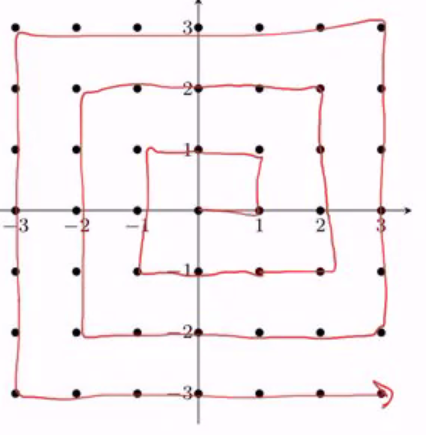
\includegraphics[scale=.25]{notes/images/picture_proof.PNG}
\end{center}
\end{example}

\begin{example}
Is $\Q$ countable or uncountable? To develop our intuition for this, let's think about the fact that we can represent a rational number as $\frac{a}{b}$ where $b \neq 0$. Now if we define our bijection as $\frac{a}{b} \to (a, b)$. We can then ignore the lower two quadrants as they are the same as other points. And then we can use a similar spiral as our previous proof to pictorially develop a bijection. We can now say that $\N, \Z, \Z \times \Z, \Q$ are all countable (all have the same cardinality. 
\end{example}

At this point you may be wondering, is everything countable? Let's look at an answer to that question. 

\begin{example}
\begin{claim}
The open interval $(0, 1)$ is uncountable. 
\end{claim}
\begin{proof}
This is often referred to as Cantor's diagonal proof (diagonalization). Let $f: \N \to (0, 1)$. We'll show that $f$ isn't surjective. Write $f(1), f(2), f(3), \dots$ as decimals not ending in repeating $9$s (think about what $\bar{.9}$ is). We can consider one such an example:
\begin{align*}
    f(1) &= .7654157\dots \\
    f(2) &= 0.1543296 \dots \\
    f(3) &= 0.5000000 \dots 
\end{align*}
We now want to construct an example that doesn't get hit by our function. Let's call this number $w$. Let $w$ be the decimal whose $n$-th digit is 
\[
\text{digit = } \begin{cases}
        5 \text{ if the $n$-th digit of $f(n)$ isn't $5$,}
        \\
        6 \text{ if otherwise.}
        \end{cases}
\]
We can start constructing our $w$ using our previous examples. We would get something like $w = 0.565 \dots$. We have that $w \in (0,1)$, but could it be equal to $f(1)$? No, because we changed a digit. This is true for all $n$ i.e. $\forall n \in \N \; w \neq f(n)$ as it has a different $n$-th digit. So, $f$ isn't surjective!
\end{proof}
\end{example}

\begin{example}
There's a precise way to measure the length of a subset of $\R$; we won't go into all of the details (this is a field of math known as measure theory), but here are some basic facts:
\begin{enumerate}
    \item The length of any subset of $\R$ is $\geq 0$.
    \item The length of an open interval $(a, b)$ is $b-a$.
    \item If $A \subseteq B$, then (length of $A$) $\leq$ (length of $B$).
    \item The length of $A \cup B$ is $\leq$ to $length(A) + length(B)$.
\end{enumerate}
Let $S$ be a countably infinite subset of $R$. What can you say about the length of $S$? Letting $S$ be such a subset of $R$. Then, there's a bijection $f: \N \to S$. Let $\epsilon > 0$. Thinking about the intervals around $f(n)$ for $n \in \N$ as being progressively tighter around $f(n)$. Let:
\begin{align*}
    I_1 &= (f(1) - \frac \epsilon 4, f(1) + \frac \epsilon 4 \\
    I_2 &= (f(2) - \frac \epsilon 8, f(2) + \frac \epsilon 8 \\
    I_3 &= (f(3) - \frac \epsilon {16}, f(3) + \frac \epsilon {16} \\
\end{align*}

Let $I = I_1 \cup I_2 \cup I_3 \cup \dots$. Then $S \subseteq I$, so $length(s) \leq length(I) \leq length(I_1) + length(I_2) + \dots$. This is equal to $\frac{\epsilon}{2} + \frac{\epsilon}{4} + \frac{\epsilon}{4} + \frac{\epsilon}{8} + \dots = \epsilon$. We have shown that the $length(s) \leq \epsilon$ for every $\epsilon > 0$, so the length of $S$ must be $0$!



We can provide another proof of this in the following way:
\begin{proof}
$(0,1)$ has length $1$, but countable subsets of $R$ have length $0$.
\end{proof}
\end{example}

\begin{example}
Let $a,b \in \R$ with $a<b$. True or false:
\begin{enumerate}
    \item There is a rational number $q$ with $a < q < b$.
    This is true. For a proof, refer to worksheet 15!
    \item There is an irrational number $r$ with $a < r < b$. 
    We can make a straightforward argument to show that this is true. Consider the fact that the length of the interval $(a,b)$ is greater than $0$. Additionally, the length of the rationals is $0$. Therefore, there must be irrational numbers in $(a, b)$.
\end{enumerate}
\end{example}

To take stock of what we saw today, we have that $\N, \Z, \Q$ all have the same cardinality and are namely countable. We saw that $(0,1)$/any open interval and $\R$ are uncountable and have the same cardinality. We will leave you with an interesting question called the Continuum hypothesis: is there a cardinality in between the integers and the reals? It has been shown to be both consistent and inconsistent i.e. unprovable. There is a continuing debate about it to this day. 
